\section{Description and Methodology}

\subsection{Theoretical background}
Sound propagates through compressable and solid media as waves, and they are often described in terms of sinusoidal plane waves. The human ear can percept frequencies ranging from 20 Hz to 20,000 Hz, the higher frequency, the higher pitch.
\begin{figure}[h]
	\centering
	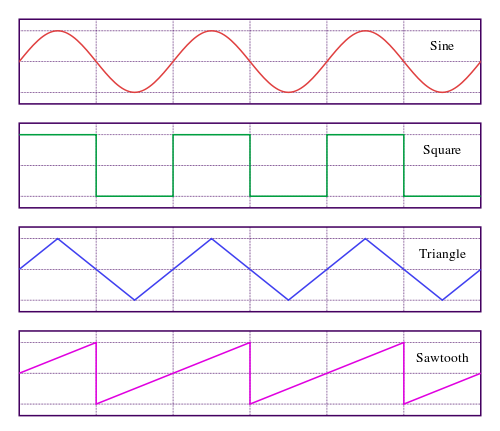
\includegraphics[width=8cm]{img/waveforms.png}
	\caption{Sine, square, triangle, and sawtooth waveforms. Figure found at \cite{wikipedia_sawtooth}.}
	\label{fig:sawtooth}
\end{figure}

In order to produce sound with the Digital-to-Analog converter, these waves need to be modeled. There are three simple ways: Square, triangle and sawtooth (see figure \ref{fig:sawtooth}). By repeatedly calculating the wave position(s) and write the result to the DAC, sound with the given frequency/frequencies are produced and can be percepted by the human ear if a headset is attached to the DAC. The more often write to the DAC, or the higher the sampling rate, the quality of the sound improves. \cite{compendium} states that a sampling rate of 48 kHz is a good reference value. 

\begin{figure}[h]
	\centering
	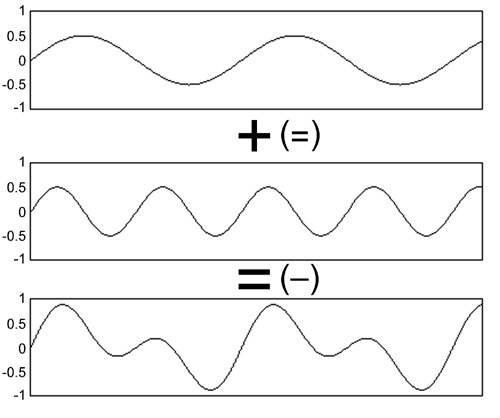
\includegraphics[width=8cm]{img/sumofsines.jpg}
	\caption{Adding sound waves together. Figure found at \cite{fourier}.}
	\label{fig:adding_waves}
\end{figure}
To play multiple frequencies together, you exploit the addititive nature of waves. You calculate each signal for a frequency independently, and then add them together (See figure \ref{fig:adding_waves}).
\subsection{Project structure}
Here is a little overview of the files in the project. There will not be a thorough explanation of the code, as it is well documented. The project consist of two parts; the C code flashed to the \boardName\ (located in \emph{code/}) and a simple python script for generating samples from sheet music (located in \emph{sampler/}).

\begin{itemize}
	\item \emph{code/dac.c} - DAC initialization.
	\item \emph{code/ex2.c} - Contains the applications entry method. Sets up all pherepials and external modules. Will configure interrupt handling.
	\item \emph{code/gpio.c} - GPIO initialization.
	\item \emph{code/interrupt\_handlers.c} - Contains interrupt procedures for timers and GPIO. Will communicate with \emph{code/sampler.c} to set sampler modes and push samples onto the DAC.
	\item \emph{code/Makefile} - Makefile for cross compiling and uploading binaries to \boardName .
	\item \emph{code/sampler.c} - Independent module for sample calculation. Will generate sample values depending on the sampler mode.
	\item \emph{code/timer.c} - High and low frequency timer setup. Also contains logic for turning the low energy timer on and off.
	\item \emph{sampler/freq.csv} - Contains frequency values for all notes.
	\item \emph{sampler/Makefile} - Will generate and concatenate several tracks into one C source file which will be included in the data segment of the code uploaded to the board.
	\item \emph{sampler/sampler.py} - Python script for generating samples from sheet music.

\end{itemize}

Most of the c source files has a corresponding header to define their external interfaces.

\subsection{Getting started}
Like last time, we initially developed a simple application with all the basics set up. The DAC, timer and GPIO was set up in the files dac.c, timer.c and gpio.c. The interrupts where handled in the interrupt\_handlers.c file. The main part of our program is the sampler.c. The interrupt handlers send and receive data to and from the sampler.c file. The gpiohandler set one of 9 modes in sampler.c and the timerhandler pulls information from the sampler program and feeds it to the dac. 

\subsection{Sampler}
As explained, all logic for calculating DAC output is located in \emph{code/sampler.h}.
\subsubsection{Sample file format}
\begin{figure}[h]
	\centering
	\begin{lstlisting}[language=C]
typedef struct sample {
	float hz;
	int ms;
} sample\_t;
	\end{lstlisting}
	\caption{Sample struct}
	\label{file_format_struct}
\end{figure}
To be able to play sound sequences, we invented our own, very simple, audio format. It consists of simple structs, each contaning frequency and duration (see figure \ref{file_format_struct}) To represent a sequence, we placed several different samples in an array. Then in the sampler\_get() function, a counter was set to increase each call. When the counter had been increased enough to call it a millisecound, the duration of the current playing sample decreased. This was because the  unit of the duration field in our sample struct where set to millisecounds.\\
\\
Now, The system supported sound-sequences, but there where no support for sound sequences with multiple tracks. To support multiple tracks, we figured the program should be able to play several samples in paralell. The one dimensional array containing samples was augmented to a two dimensional array. Also the variables containing the threshold and the remaining time for the current frequency was set to arrays. Now, all tracks would be updated every millisecound. To play different samples over each other, the different thresholds where scaled, added together and scaled once more before being sendt to the dac.\\
\\
All functionality that generates sound is found in the sampler.c file. To create sound, we had one variable increase \samplerPullsPerSecound times per secound. When this variable reached a threshold, it would be set to zero. This variable would the be sent to the dac, wich would  then produce a constant tone. TODO: Skriv noe om hvordan pitch ble kontorollert. \\

\subsubsection{Maintaining wave state}

\subsubsection{Managing several tracks}

\subsection{Generating samples}
Our file format for the samples is really easy to deal with, as the only information you need to supply is the frequency and duration of the sample. However, we wanted to easier be able to play melodies in sheet music, so we made a python script simplifying this task for us. The python script accepts csv file format, which contains the following data:
\begin{itemize}
	\item Track name.
	\item Variable names.
	\item Beats per minute.
	\item List of note keys with corresponding length.
\end{itemize}

Please see the code for more details, and the corresponding Makefile to see how the script is used.

\subsection{Low energy timer and sleep modes}

To make our program more energy efficient, we made use of a low energy timer. This runs on a low frequency clock and, compared to the high frequency clock TIMER1 which have a frequency of 48 MHz, the low energy clock have a frequency of only 32 kHz. We expect that this timer should save some power as it runs on a lower frequency. \\

We did the following to enable the low energy timer:

\begin{enumerate}
	\item {Write 16 to CMU\_HFCORECLKEN0 to enable clock for low energy timers.}
	\item {Write 64 to CMU\_OSCENCMD to enable low energy oscilator LFRCO used by LFACLK (see figure 11.1 in the efm32gg reference manual). LFACLK is the clock used by LETIMER0.}
	\item {Write 4 to CMU\_LFACLKEN0 to enable the clock for the LETIMER0.}
	\item {Write 512 LETIMER0\_CTRL to set the top of the timer to the register COMP0. This makes it possible to use the LETimer as a regular timer. Since COMP0 is the top value, it will be reffered to as LETIMER0\_TOP.}
	\item {Write the the top value to LETIMER0\_TOP.}
	\item {Enable interrupts by writing 1 to LETIMER0\_IEN.}
	\item {Start the timer by writing 1 to LETIMER\_CMD.} 
\end{enumerate}

An interrupt is triggered each time the timer is done counting. In our code this is ones every tick. When an interrupt is triggered the LETIMER0\_IRQHandler()-routine in \emph{interrupt\_handlers.c} is called. This writes the correct output to the DAC. \\

If we are done playing a track there is no need to output anything to the DAC. Therefore the sampler signals the interrupt-routine if we are done playing a sound. The next interrupt we turn of the timer by calling stopLETimer()-routine in \emph{interrupt\_handlers.c}. This turns of the low frequency clock LFACLK.
\\This makes it easy for us to enter lower energy modes when we are not playing any sound. To enter EM2, we enable deepsleep mode in the same fassion as in exercise 1 via the routine setupEM2() in \emph{ex2.c}. Since we also disable the low frequency clocks when not playing sound, we are enabling EM3. \\
When a button is pressed, the sampler is filled with data again and it signals the timer to start with the startLETimer()-routine in \emph{interrupt\_handler.c}. This turns on the low frequency clock LFACLK. \\
 
When we are feeding the DAC with samples, we are in EM0 which should consume alot energy when the CPU is feeding the DAC. Since the CPU cannot feed the DAC and sleep at the same time, we had to look for solutions when we do not have any samples to output. therefore we choosed to bring the system into EM3 when nothing is to be done, to minimize the energy consumed by the system. we concluded that since the low energy timer is active, the CPU will always be awake even though the sampler is empty. therefore we needed to make sure that the timer was disabled when there was no new samples to output to the DAC. in our code EM3 is the energy mode that allows us to do just that, making EM1 and EM2 undesirable as the low frequenzy clock LFACLK is still active. \\

The problem with this solution is that it does not scale. If any other low frequent peripheral is using the LFACLK, we need to most likely need to rewrite the timer start- and stop-routines. We would have to make the timer start and stops more specific, and write to the registers of the low energy timer instead. The highest energy mode we could enter, if we just turned off the timer and not the low frequency clock, would be EM2. Since we only use the low energy timer in this assignment, we stick with our first solution to the energy consumption problem. 
 



